\documentclass[11pt]{article}
\usepackage{../EllioStyle}
\usepackage{listings}

\definecolor{codegreen}{rgb}{0,0.6,0}
\definecolor{codegray}{rgb}{0.5,0.5,0.5}
\definecolor{codepurple}{rgb}{0.58,0,0.82}
\definecolor{backcolour}{rgb}{0.95,0.95,0.92}

\graphicspath{ {imgs/} }

\title{Homework 3}
\author{Elliott Pryor}
\date{11 November 2023}

\rhead{Homework 3}

\begin{document}
\maketitle

My work can be found on my github:
\href{https://github.com/ElliottP-13/DeepRL-Course/tree/main/hw1}{https://github.com/ElliottP-13/DeepRL-Course}.

\large{\textbf{Problem 1}}
Evaluation on Ms Pacman. The results can be seen in Figure \ref{fig:q1}.

\begin{figure}[h]
    \centering
    \begin{subfigure}{.75\textwidth}
        \centering
        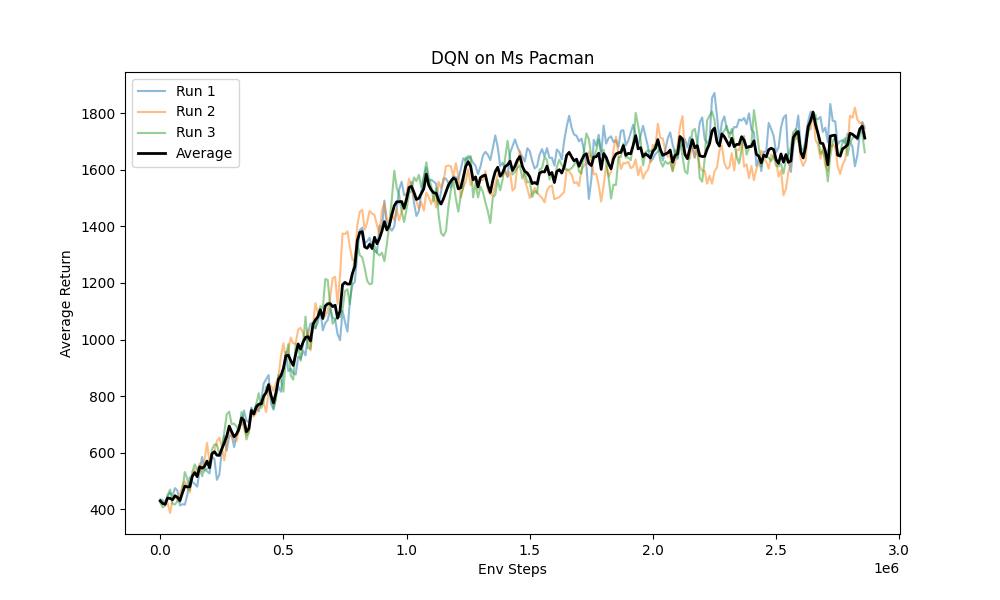
\includegraphics[width=.95 \linewidth]{hw3_q1.png}
        \caption{Average reward per episode.}
        \label{fig:}
    \end{subfigure}
    \begin{subfigure}{.75\textwidth}
        \centering
        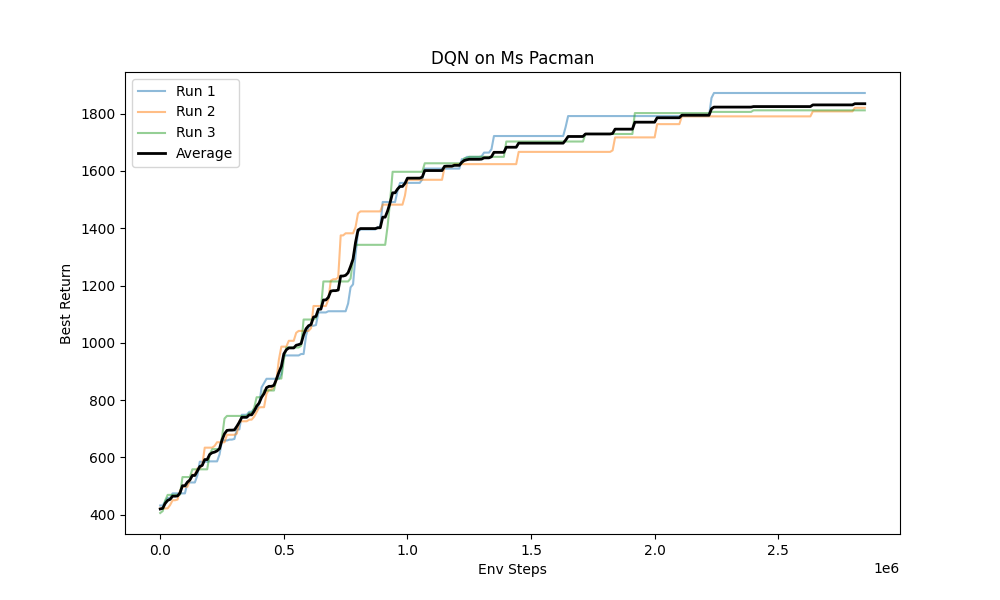
\includegraphics[width=.95 \linewidth]{hw3_q1_best.png}
        \caption{Best reward per episode.}
        \label{fig:}
    \end{subfigure}
    \caption{Performance of DQN on Ms Pacman}
    \label{fig:q1}
\end{figure}

\large{\textbf{Problem 2}}
Double Deep Q learning.

We see in Figure \ref{fig:q2_all} that DQN and DDQN perform similarly on Lunar Lander. DDQN does slightly better, but the difference is not significant. We see that both DQN and DDQN converge to a similar value.
DQN actually performes slightly better than DDQN, but the difference is not significant. We see that both DQN and DDQN converge to a similar value.
DDQN also has lower variance in performance, which may be preferable.

\begin{figure}
    \begin{subfigure}{.5\textwidth}
        \centering
        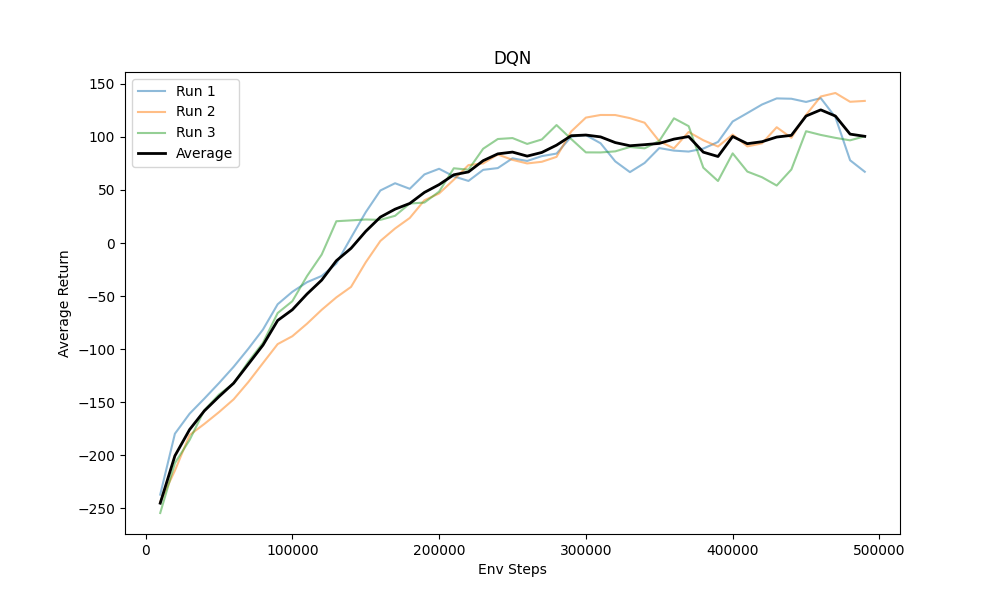
\includegraphics[width=.95 \linewidth]{hw3_q2_dqn.png}
        \caption{DQN on Lunar Lander}
        \label{fig:}
    \end{subfigure}
    \begin{subfigure}{.5\textwidth}
        \centering
        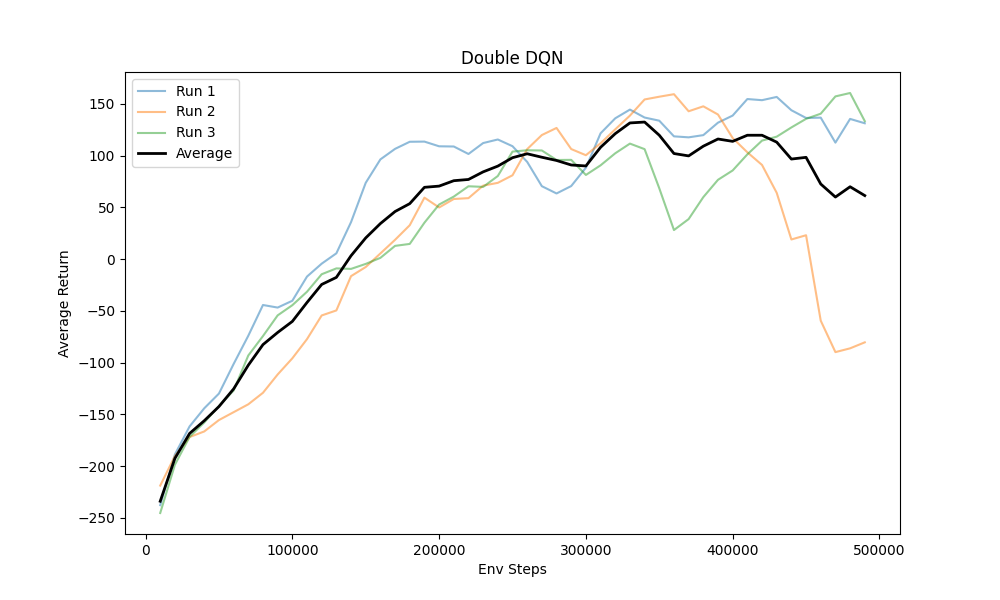
\includegraphics[width=.95 \linewidth]{hw3_q2_ddqn.png}
        \caption{DDQN on Lunar Lander}
        \label{fig:}
    \end{subfigure}
    \caption{Performance of DQN and DDQN on Lunar Lander}
\end{figure}



\begin{figure}[h] 
    \centering
    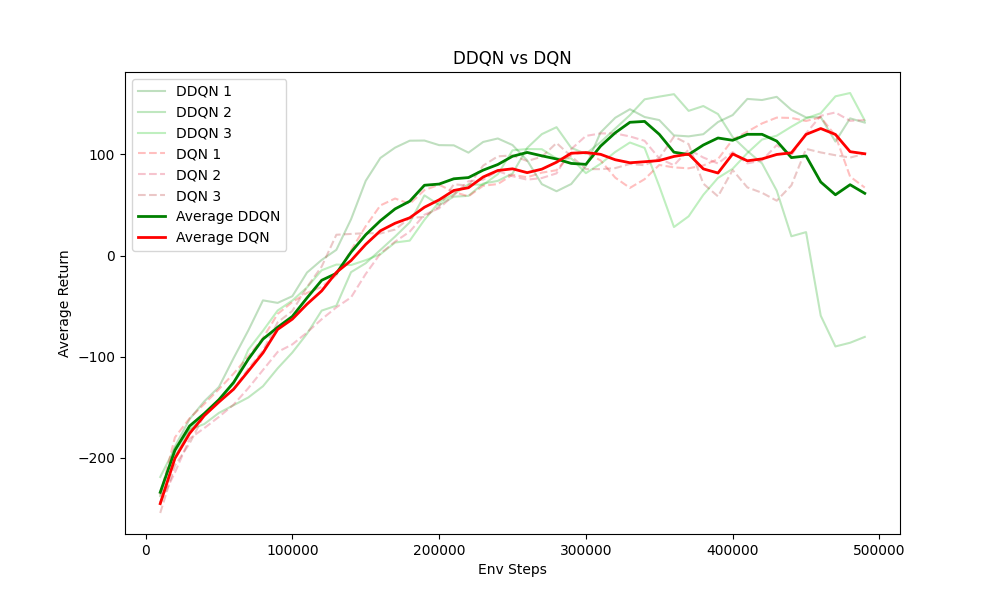
\includegraphics[width=0.95 \linewidth]{hw3_q2_all.png}
    \caption{DQN v DDQN on Lunar Lander.}
    \label{fig:q2_all}
\end{figure}


\large{\textbf{Problem 4}}
Actor critic results can be seen in Figure \ref{fig:ac}.
We can see that Actor Critic can fully solve the problem in very few iterations.
About 40,000 iterations it reaches max performance. However, in homework 2,
the vanilla policy gradient did this in about 1000 environment steps. 
This is probably because vanilla policy gradient is lighter and able to more quickly solve this easy problem.

\begin{figure}[h] 
    \centering
    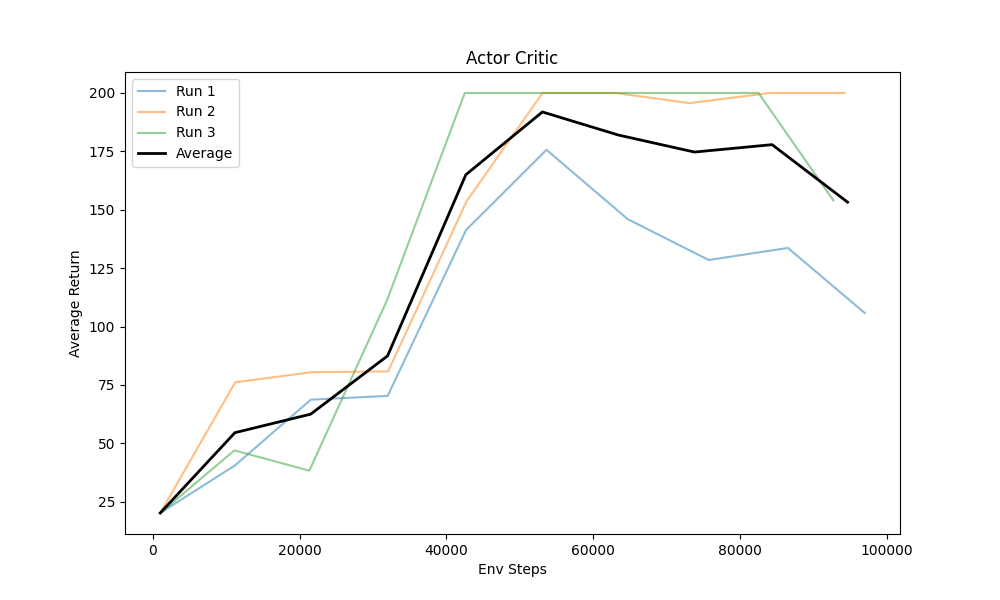
\includegraphics[width=0.95 \linewidth]{hw3_q4.png}
    \caption{Performance of Actor Critic on cartpole.}
    \label{fig:ac}
\end{figure}

\end{document}